% Clase del documento
\documentclass[12pt, letterpaper]{article}

% Definicion del preambulo
% Para insertar imágenes
\usepackage{graphicx}

% Para tener referencias
\usepackage{hyperref}

% Para poner matemáticas
\usepackage{amsthm, amssymb}

\setlength {\marginparwidth }{2cm}
% Comentarios en pdf
\usepackage{todonotes}

% Matrices
\usepackage{amsmath}

% Para poner definiciones con color
\usepackage[most]{tcolorbox}

% Colores
\usepackage{xcolor}

% Quita sangrías/Pone saltos en párrafos
%\usepackage{parskip}

% Español
\usepackage[spanish]{babel}

% imagenes svg
\usepackage{svg}

% para insertar imágenes en una posición estricta
\usepackage{float}

% Definición personalizada de tcolorbox
\newtcolorbox{miDefinicion}[2][]{
  colback=teal!5!white,
  colframe=teal!75!black,
  coltitle=white,
  fonttitle=\bfseries,
  title=Definición: #2,
  arc=2mm,
  boxrule=0.8pt,
  enhanced,
  drop shadow,
  #1
}

% Para poner call outs chidos
\usepackage{mdframed}
% Definimos el estilo del callout con línea a la izquierda
\newmdenv[
  topline=false,      % Quita la línea superior
  bottomline=false,   % Quita la línea inferior
  rightline=false,    % Quita la línea derecha
  leftline=true,      % Activa solo la línea izquierda
  linecolor=cyan,     % Color de la línea (puedes usar blue, red, etc.)
  linewidth=3pt,      % Grosor de la línea
  innerleftmargin=10pt, % Espacio entre la línea y el texto
  innerrightmargin=0pt,
  innertopmargin=0pt,
  innerbottommargin=0pt
]{miencuadre}

% Titulo, autor y fecha
\title{\textbf{\textcolor{cyan}{Paquitos}}}
\author{Ricardo Victoria}
\date{Septiembre 2027}

% Inicio del documento
\begin{document}

% Insertamos el preambulo
\maketitle

% Insertamos secciones
\section*{Introducción}
En este documento aprenderemos cómo se arman los paquitos. Dado que todo eso ocupa varios conceptos, acá los explicaremos de manera superficial. 

\section{Armado}
A excepción de unos puntos que mencionaremos adelante, seguir las instrucciones indicadas en la \href{https://osoyoo.com/2022/07/05/v2-metal-mecanum-wheel-robotic-lesson1-robot-car-assembly-model-2021006600/}{lección 1 de la página de Osoyoo para el M2.0 Metal Mecanum Wheel Robotic}, a la cual se puede acceder haciendo click \href{https://osoyoo.com/2022/07/05/v2-metal-mecanum-wheel-robotic-lesson1-robot-car-assembly-model-2021006600/}{acá}. También pueden ver un \href{https://youtu.be/6euit9dwO3s?si=XZ8wJ6h1Dq4ReS38}{video de cómo se arma} haciendo \href{https://youtu.be/6euit9dwO3s?si=XZ8wJ6h1Dq4ReS38}{click acá}. Esa lección indica cómo armar el esqueleto base de nuestros Paquitos. 

Nuestros Paquitos van a cambiar en los siguientes puntos.

No hay que hacer caso sobre dónde poner las baterías. En la página se pide que se coloquen sobre la tabla de acrílico superior, pero nosotros las vamos a colocar sobre la tabla inferior, como se ve en la foto de la figura \ref{fig:lugar-baterias1}.

\begin{figure}[htbp]
    \centering
    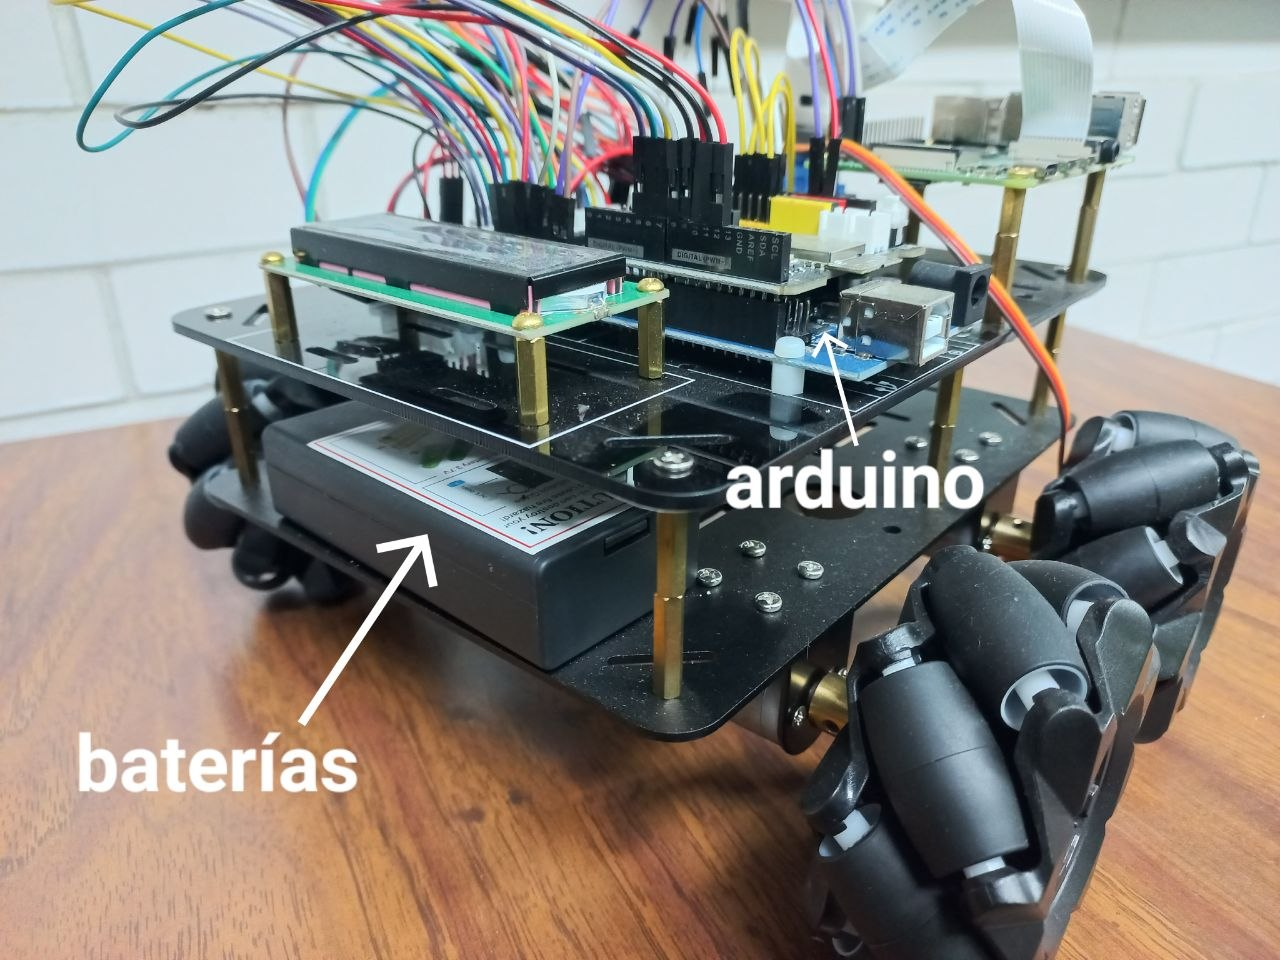
\includegraphics[width=0.5\textwidth]{imagenes/lugar-baterias.jpg}
    \caption{Baterías sobre la tabla de acrílico inferior.}
    \label{fig:lugar-baterias1}
\end{figure}

Luego, con un taladro, perforaremos cuatro agujeros sobre la tabla de acrílico superior para poner una raspberry pi. En la foto de la figura \ref{fig:lugar-raspberry} se aprecia dónde debe quedar la raspberry pi, y por tanto, dónde hacer los agujeros. 

\begin{figure}[htbp]
    \centering
    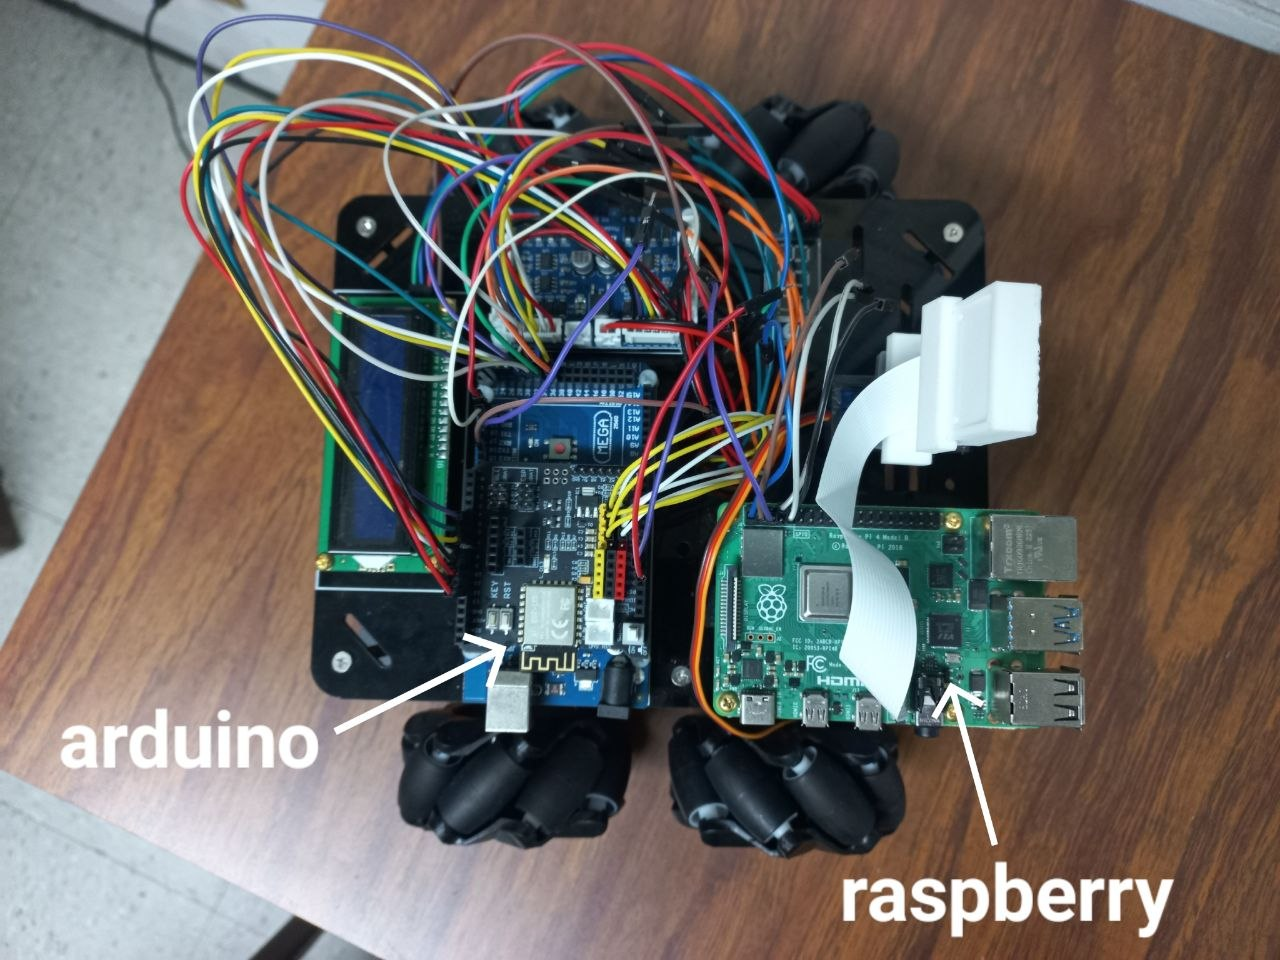
\includegraphics[width=0.5\textwidth]{imagenes/lugar-raspberry.jpg}
    \caption{Ubicación de la raspberry sobre la tabla superior de acrílico.}
    \label{fig:lugar-raspberry}
\end{figure}

Además, vamos a cambiar bastante el acomodo de los cables del arduino. Así que a continuación se explicará cómo debemos conectar esa parte. 

\subsection{Cables del arduino, controlador y motores}
En la lección 1 de la página de osoyoo, no se conectan los encoders integrados en los motores al arduino. Nosotros sí los vamos a conectar. Para conectarlos, tendremos que cambiar casi todo el cableado del arduino que originalmente se indicaba en la página. 

Cada motor tiene seis pines: S2 (sensor 2 del encoder), S1 (sensor 1 del encoder), GND (tierra del encoder), VCC (voltaje del enconder), M- (negativo del motor), M+ (positivo del motor). Por tanto, de cada motor salen 6 cables. 

A continuación explicaremos cómo conectar los pines M- y M+ de cada motor al controlador \textit{Osoyoo Model Y 2.0} (pues no se hace exactamente como en la página).

%Los pines M- y M+ (que corresponden al motor) sí deben de estar conectados al controlador \textit{Osoyoo Model Y 2.0} como se indica en la página. 

\begin{miencuadre}
    El \textit{Osoyoo Model Y 2.0} es un controlador fabricado por Osoyoo que sirve como intermediario (porque es un controlador de hardware) entre el arduino y los motores. Este controlador recibe señales de alto nivel del arduino, y las transforma en señales de bajo nivel (voltaje crudo) que los motores entienden para saber cómo moverse.     
\end{miencuadre}

Para el motor delantero izquierdo, los pines M- y M+ se conectarán en la sección \textbf{ACK1} del controlador. Para el motor delantero derecho, los pines M- y M+ se conectarán en la sección \textbf{ACK3} del controlador. Para el motor trasero izquierdo, los pines M- y M+ se conectarán en la sección \textbf{BK1} del controlador. Para el motor trasero derecho, los pines M- y M+ se conectarán en la sección \textbf{BK3} del controlador.

Por otro lado, los pines VCC y GND (de los motores) los vamos a conectar a las líneas de 5V y GND del shield del arduino, respectivamente. La línea de 5V es la única parte de color rojo del shield, la línea de GND es la línea de color negro que está junto a la línea de 5V.

Los pines S1 y S2 (de los motores) los vamos a conectar a pines digitales del arduino. 

\begin{miencuadre}
    Los pines digitales sólo manejan dos valores: HIGH y LOW (1 y 0). Los pines S1 y S2 van a pasar de LOW a HIGH cuando su encoder correspondiente detecte un pulso en el giro de los motores (y también de las ruedas, porque están pegadas a los motores). Cuando el pulso pase, entonces los pines pasarán de HIGH a LOW. 
\end{miencuadre}

Para el motor frontal derecho, su pin S1 se conectará al pin 30 del arduino, y su pin S2 se conectará al pin 32 del arduino. Para el motor frontal izquierdo, su pin S1 se conectará al pin 31 del arduino, y su pin S2 se conectará al pin 33 del arduino. Para el motor trasero derecho, su pin S1 se conectará al pin 34 del arduino, y su pin S2 se conectará al pin 36 del arduino. Finalmente, para el motor trasero izquierdo, su pin S1 se conectará al pin 35 del arduino, y su pin S2 se conectará al pin 37 del arduino. Estas conexiones se resumen en el cuadro \ref{tab:conexiones-encoders}.

\begin{table}[h]
    \centering
    \begin{tabular}{|l|c|c|}
        \hline
        \textbf{Motor} & \textbf{Pin S1} & \textbf{Pin S2} \\ \hline
        Frontal Derecho   & Pin 30 arduino & Pin 32 arduino\\ 
        Frontal Izquierdo & Pin 31 arduino & Pin 33 arduino\\ 
        Trasero Derecho   & Pin 34 arduino & Pin 36 arduino\\ 
        Trasero Izquierdo & Pin 35 arduino & Pin 37 arduino\\ \hline
    \end{tabular}
    \caption{Conexiones Encoders-Arduino}
    \label{tab:conexiones-encoders}
\end{table}

También vamos a cambiar las conexiones que se indican en la página sobre las secciones M\_A y M\_B del controlador \textit{Osoyoo Model Y 2.0}. Para M\_A, el pin ENB (el del cable rojo) del controlador se conectará al pin pwm 10 del arduino, el pin IN4 (el del cable blanco) del controlador se conectará al pin digital 29 del arduino, el pin IN3 (el del cable amarillo) del controlador se conectará al pin digital 28 del arduino, el pin IN2 (el del cable verde) del controlador se conectará al pin digital 27 del arduino, el pin IN1 (el del cable morado) del controlador se conectará al pin digital 26 del arduino, y el pin ENA (el del cable negro) del controlador se conectará al pin pwm 9 del arduino. En el cuadro \ref{tab:conexiones-ma} se resumen estas conexiones. Para M\_B, el pin ENB (el del cable rojo) del controlador se conectará al pin pwm 12 del arduino, el pin IN4 (el del cable blanco) del controlador se conectará al pin digital 25 del arduino, el pin IN3 (el del cable amarillo) del controlador se conectará al pin digital 24 del arduino, el pin IN2 (el del cable verde) del controlador se conectará al pin digital 23 del arduino, el pin IN1 (el del cable morado) del controlador se conectará el pin digital 22 del arduino, y el pin ENA (el del cable negro) del controlador se conectará al pin pwm 11 del arduino. En el cuadro \ref{tab:conexiones-mb} se resumen estas conexiones.

\begin{table}[h]
    \centering
    \begin{tabular}{|l|l|}
        \hline
        \textbf{Pines Sección M\_A Controlador} & \textbf{Pin Arduino} \\ \hline
        ENB (Cable rojo)               & Pin PWM 10          \\ 
        IN4 (Cable blanco)             & Pin digital 29      \\ 
        IN3 (Cable amarillo)           & Pin digital 28      \\ 
        IN2 (Cable verde)              & Pin digital 27      \\ 
        IN1 (Cable morado)             & Pin digital 26      \\ 
        ENA (Cable negro)              & Pin PWM 9           \\ \hline
    \end{tabular}
    \caption{Conexiones Controlador M\_A-Arduino}
    \label{tab:conexiones-ma}
\end{table}

\begin{table}[h]
    \centering
    \begin{tabular}{|l|l|}
        \hline
        \textbf{Pines Sección M\_B Controlador} & \textbf{Pin Arduino} \\ \hline
        ENB (Cable rojo)               & Pin PWM 12          \\ 
        IN4 (Cable blanco)             & Pin digital 25      \\ 
        IN3 (Cable amarillo)           & Pin digital 24      \\ 
        IN2 (Cable verde)              & Pin digital 23      \\ 
        IN1 (Cable morado)             & Pin digital 22      \\ 
        ENA (Cable negro)              & Pin PWM 11          \\ \hline
    \end{tabular}
    \caption{Conexiones Controlador M\_B-Arduino}
    \label{tab:conexiones-mb}
\end{table}

En la siguiente sección, veremos cómo establecer una conexión i2c entre el arduino y la raspberry.

\subsection{Conexión i2c}
Para un Paquito, es necesario que su \textbf{arduino} y su \textbf{raspberry pi} estén comunicados entre sí. Necesitamos que la \textbf{raspberry pi} haga cálculos a alto nivel, y que el \textbf{arduino} haga cálculos a un bajo nivel. Para lograr esta comunicación, utilizaremos un protocolo llamado \textbf{i2c}.

Usualmente en una comunicación que utiliza el protocolo \textbf{i2c} sólo necesitas conectar ciertos pines directamente de un dispositivo a otro. Sin embargo, resulta que la raspberry pi y el arduino trabajan con un voltaje de lógica diferente. Por tanto, necesitamos de un pequeño chip conversor en medio de la comunicación i2c para que los dispositivos no se quemen.

\begin{miencuadre}
    El voltaje de lógica (lógica de control) de un dispositivo es la cantidad de voltaje con la que trabaja una placa. Es el rango de tensión eléctrica que representa un cero (0) o un uno (1) en circuitos digitales. [1] La raspberry pi de un Paquito trabaja con una lógica de voltaje de 3.3V (se ocupan 3.3V aproximadamente para representar un 1), mientras que el arduino de un Paquito trabaja con una lógica de voltaje de 5V (se ocupan 5V aproximadamente para representar un 1).
\end{miencuadre}

Este chip conversor que se usa para los paquitos es el \textit{4-Channel Bidirectional Logic Level Converter 5V to 3.3V. (Level Shifter)}, y se puede ver el la figura \ref{fig:level-shifter}. Como se puede ver en la figura \ref{fig:level-shifter}, este chip tiene de un lado marcas que empiezan con \textit{HV}, y de otro lado marcas que empiezan con \textit{LV}. Las letras \textit{HV} significan HIGH VOLTAGE, miestras que las letras \textit{LV} significan LOW VOLTAGE. Del lado de HIGH VOLTAGE se conectará la placa con la lógica de voltaje más alta (el arduino), mientras que del lado de LOW VOLTAGE se conectará la placa con la lógica de voltaje más baja (la raspberry). 

\begin{figure}[htbp]
    \centering
    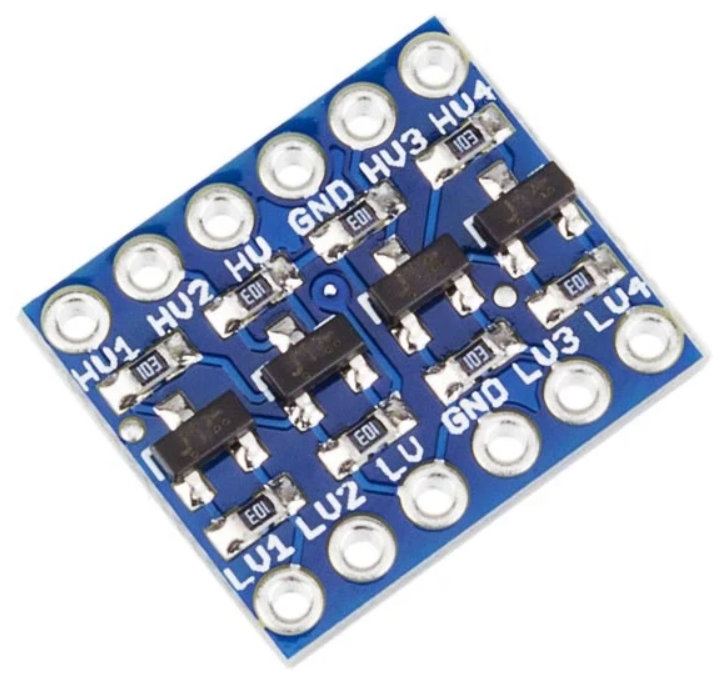
\includegraphics[width=0.5\textwidth]{imagenes/level-shifter.png}
    \caption{Chip conversor para Paquitos.}
    \label{fig:level-shifter}
\end{figure}

Entonces, para iniciar una comunicación i2c, debemos de conectar ambas placas de la siguiente manera:
\begin{enumerate}
    \item Conectar el pin SDA de la raspberry al pin LV1 del chip conversor. Luego conectar el pin HV1 del chip conversor al pin SDA del arduino.
    \item Conectar el pin SCL de la raspberry al pin LV2 del chip conversor. Luego conectar el pin HV2 del chip conversor al pin SCL del arduino.
    \item Conectar un pin GND de la raspberry al pin GND del chip conversor que está del lado de los pines LV. Luego conectar el pin GND del chip conversor que está del lado de los pines HV, a un pin de GND del arduino.
    \item Conectar un pin de 3.3V de la raspberry al pin LV del chip conversor. Luego conectar el pin HV del chip conversor a un pin de 5V del arduino.
\end{enumerate}

Esta conexión se resume en el cuadro \ref{fig:cserial}, y se puede ilustra en la figura \ref{fig:i2c}.

\begin{table}[h]
    \centering
    \begin{tabular}{|c|c|c|c|}
        \hline
        Raspberry Pi & Conversor (LV) & Conversor (HV) & Arduino \\
        \hline
        SDA & LV1 & HV1 & SDA \\
        SCL & LV2 & HV2 & SCL \\
        GND & GND (LV) & GND (HV) & GND \\
        3.3V & LV & HV & 5V \\
        \hline
    \end{tabular}    
    \caption{Conexión Serial.}
    \label{fig:cserial}
\end{table}



\begin{figure}[htbp]
    \centering
    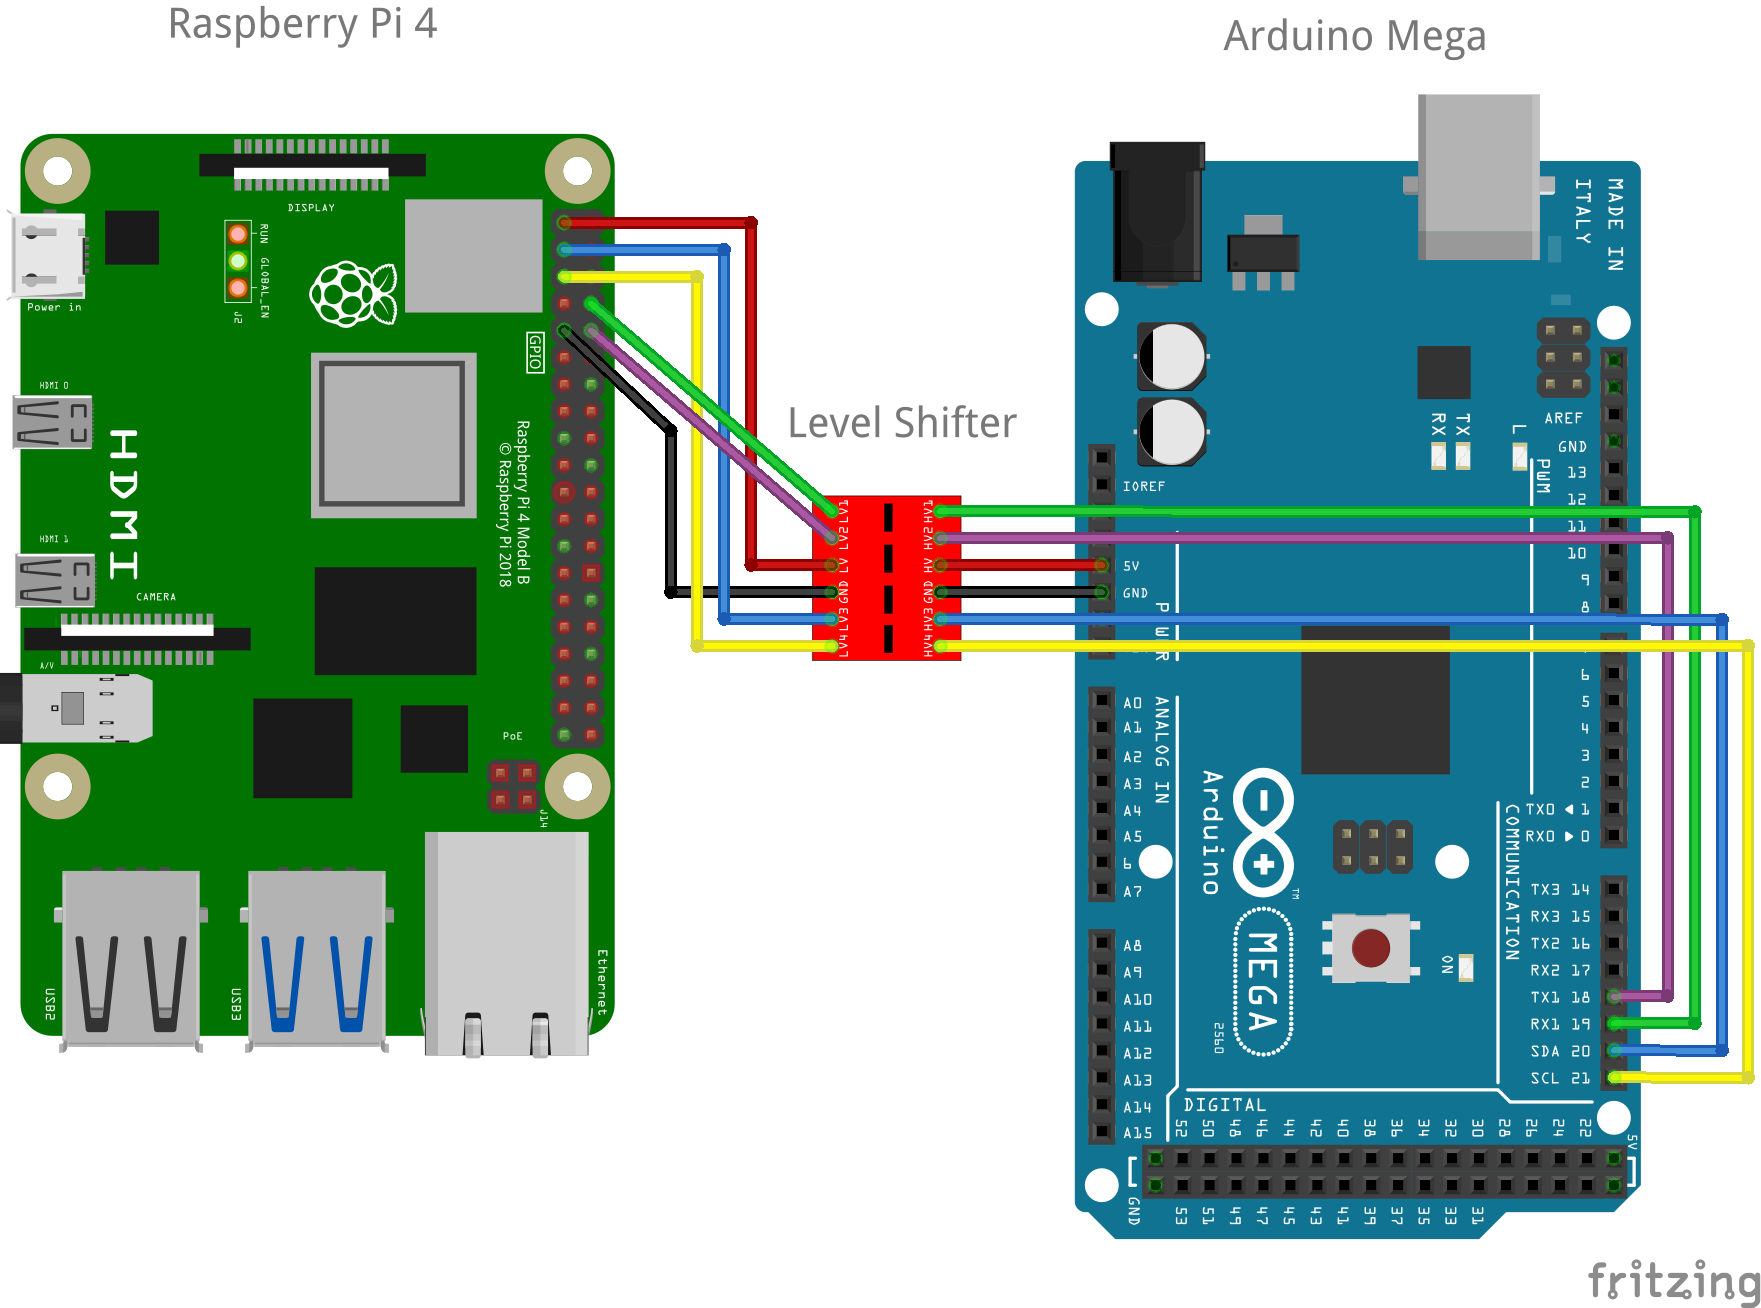
\includegraphics[width=0.7\textwidth]{imagenes/i2c-connection_bb.png}
    \caption{Conexión i2c y serial.}
    \label{fig:i2c}
\end{figure}




\subsection{Conexión Serial Arduino-Raspberry}

Para comunicar la información de los encoders a la raspberry pi, utilizaremos una conexión serial entre el arduino y la raspberry. Para ello, utilizaremos los pines RX y TX del arduino. Y, volveremos a usar el chip conversor. 

Conectamos el pin RX del arduino con el pin HV3 del chip conversor, luego conectaremos el pin LV3 de chip conversor con el pin TX de la raspberry. Conectamos el pin TX del arduino con el pin HV4 del chip conversor, luego, conectamos el pin LV4 del chip conversor con el pin RX de la raspberry. Estas coneciones se resumen en el cuadro \ref{tab:cserial}; y se ilustran en la figura \ref{fig:i2c}.

\begin{table}[htpb]
    \centering
    \renewcommand{\arraystretch}{1.3}
    \begin{tabular}{@{}llll@{}}
        \toprule
        \textbf{Pin Arduino (5V)} & \textbf{Conversor (HV)} & \textbf{Conversor (LV)} & \textbf{Pin Raspberry (3.3V)} \\
        \midrule
        RX & HV3 & LV3 & TX \\
        TX & HV4 & LV4 & RX \\
        \bottomrule
    \end{tabular}
    \caption{Resumen de conexiones seriales (UART) entre Arduino y Raspberry Pi usando el conversor.}
    \label{tab:cserial}
\end{table}



\subsection{Display LCD}

También vamos a añadir a nuestros Paquitos un Display LCD (en adelante display).

En la tabla de acrílico superior, del lado del arduino, en el espacio que queda, vamos a hacer unas perforaciones con el taladro y fijaremos el display. 

El display también se conectará con la raspberry usando el protocolo i2c. Así que vamos a conectarlos de la siguiente forma. 

El display tiene cuatro pines: \textbf{GND}, \textbf{VCC}, \textbf{SDA} y \textbf{SCL}. Dado que el display tiene un voltaje de lógica de 5V, entonces vamos a tener que usar el chip conversor para la comunicación. Vamos a conectar los pines del display del lado de HIGH VOLTAGE del chip conversor. Conectaremos el pin GND del display con el GND del HV del chip conversor, luego el pin VCC del display con el pin HV del chip conversor, luego el pin SDA del display con el pin HV1 del chip conversor, y finalmente conectaremos el pin SCL del display con el pin HV2 del chip conversor. Estas conexiones se resumen en el cuadro \ref{tab:conexiones_display}.

\begin{table}[htpb]
    \centering
    \renewcommand{\arraystretch}{1.3}
    \begin{tabular}{@{}ll@{}}
        \toprule
        \textbf{Pin del Display} & \textbf{Pin del Chip Conversor (High Voltage)} \\
        \midrule
        GND & GND (HV) \\
        VCC & HV \\
        SDA & HV1 \\
        SCL & HV2 \\
        \bottomrule
    \end{tabular}
    \caption{Resumen de conexiones entre el display (lógica 5V) y el conversor de nivel lógico.}
    \label{tab:conexiones_display}
\end{table}


\subsection{Misceláneos}

\subsubsection{Conectar Tierras}

Es importante conectar las tierras (GND) de nuestros dispositivos. Hasta este punto, sólo falta conectar un pin GND del arduino con un pin negativo del Model Y board. 

\subsubsection{Bocina}

Colocar la bocina en algún espacio sobre el acrílico superior. Conectar un pin de la bocina con el pin 8 del arduino. El otro pin creo que es conectarlo a tierra del arduino.

\subsubsection{Cámara}

Tener el módulo de cámara para la raspberry pi (es decir, tener la cámara), el cuál se ilustra en la figura \ref{fig:cam}. Luego insertarla en el puerto del módulo de cámara, este puerto se ilustra en la figura \ref{fig:pcam}. Imágenes tomadas de \href{https://projects.raspberrypi.org/en/projects/getting-started-with-picamera/1URL}{https://projects.raspberrypi.org/en/projects/getting-started-with-picamera/1}.

\begin{figure}[htbp]
    \centering
    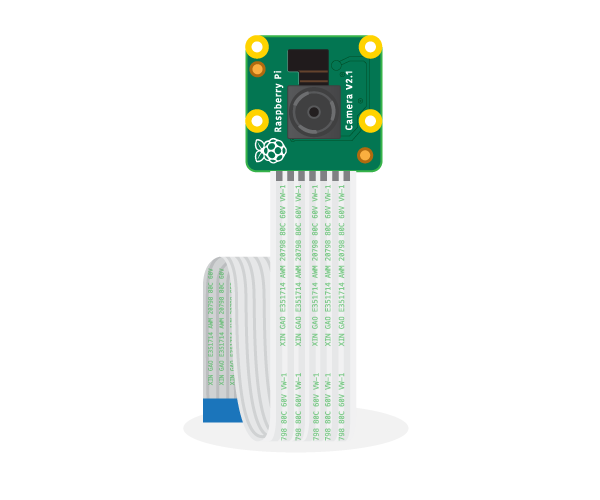
\includegraphics[width=0.3\textwidth]{imagenes/camera-module.png}
    \caption{Módulo de cámara para la raspberry pi.}
    \label{fig:cam}
\end{figure}

\begin{figure}[htbp]
    \centering
    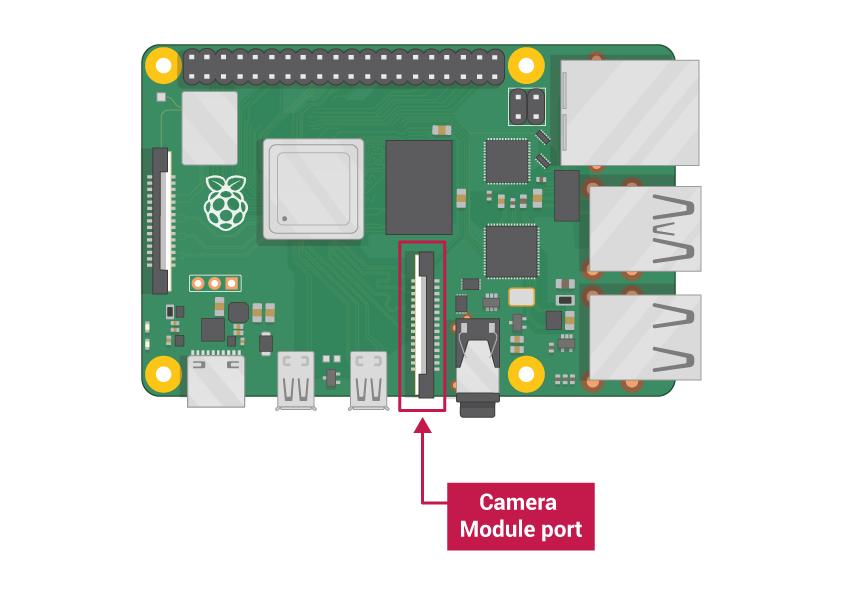
\includegraphics[width=0.3\textwidth]{imagenes/pi4-camera-port.png}
    \caption{Puerto para el módulo de cámara}
    \label{fig:pcam}
\end{figure}


\section{Referencias}
[1] https://www.sciencedirect.com/topics/computer-science/logic-level


\end{document}
